\documentclass[tikz,border=5pt]{standalone}
\usepackage{tikz}
\usetikzlibrary{3d}

\begin{document}

\tikzset{every picture/.style={line width=1.5pt}} %set default line width to 0.75pt        

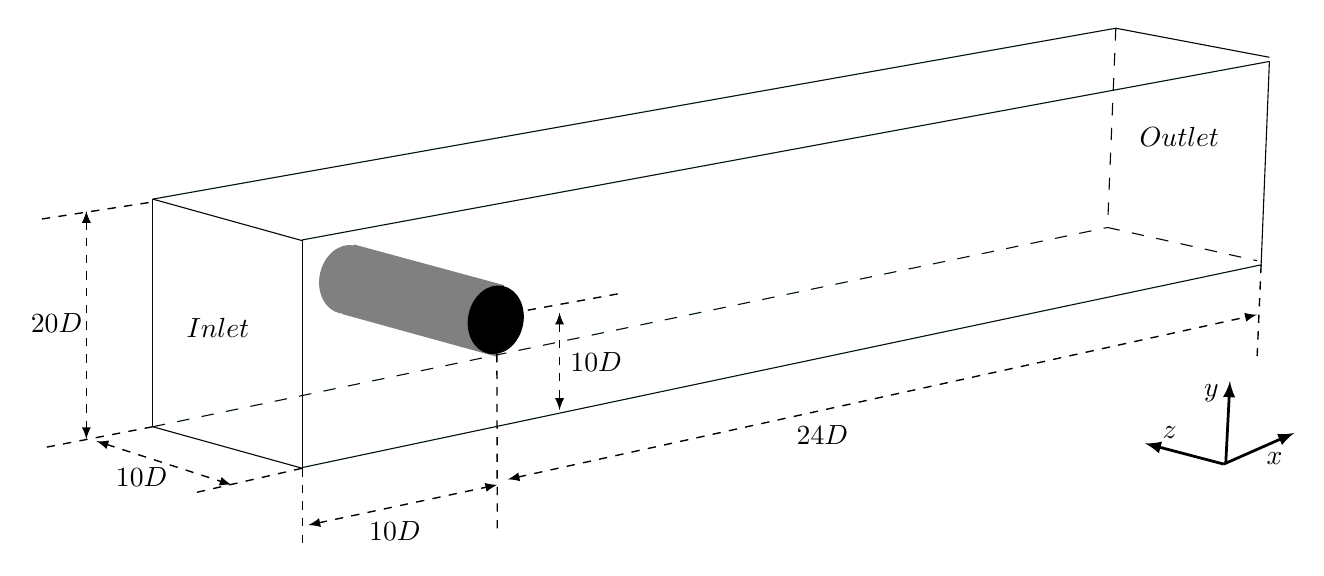
\begin{tikzpicture}[x=0.75pt,y=0.75pt,yscale=-1,xscale=1]

	%%RECTANGLE---------------------------------------------
	%%Top right line
	\draw [color={rgb, 255:black, 233; green, 17; blue, 17 }  ,draw opacity=1 ]   (142,262) -- (608,176) ;
	%%Top right line
	\draw [color={rgb, 255:black, 233; green, 17; blue, 17 }  ,draw opacity=1 ]   (70,242.33) -- (534,160) ;
	%%Top front
	\draw [color={rgb, 255:black, 245; green, 9; blue, 9 }  ,draw opacity=1 ]   (70,242.33) -- (142,262.33);
	%%Top back line
	\draw [color={rgb, 255:black, 245; green, 9; blue, 9 }  ,draw opacity=1 ]   (534,160) -- (608,174) ;

	%%Bottom right line
	\draw [color={rgb, 255:black, 233; green, 17; blue, 17 }  ,draw opacity=1 ]   (142,371.67) -- (604,274) ;
	%%Bottom front line
	\draw [color={rgb, 255:black, 245; green, 9; blue, 9 }  ,draw opacity=1 ]   (70,352) -- (142,372) ;
	%Bottom back
	\draw [color={rgb, 255:black, 245; green, 9; blue, 9 }  ,draw opacity=1 ] [dash pattern={on 4.5pt off 4.5pt}]  (530,256) -- (602,272) ;
	%front left
	\draw [color={rgb, 255:black, 223; green, 10; blue, 10 }  ,draw opacity=1 ]   (70,242.33) -- (70,352) ;
	%Front right
	\draw [color={rgb, 255:black, 223; green, 10; blue, 10 }  ,draw opacity=1 ]   (142,262) -- (142,371.67) ;
	%back left
	\draw [color={rgb, 255:black, 223; green, 10; blue, 10 }  ,draw opacity=1 ] [dash pattern={on 4.5pt off 4.5pt}]  (534,160) -- (530,256) ;
	%back right
	\draw [color={rgb, 255:black, 223; green, 10; blue, 10 }  ,draw opacity=1 ]   (608,176) -- (604,274) ;
	%bottom left 
	\draw [color={rgb, 255:black, 233; green, 17; blue, 17 }  ,draw opacity=1 ] [dash pattern={on 4.5pt off 4.5pt}]  (70,352) -- (530,256) ;

	%%CYLINDER---------------------------------------------
	%	\draw [color={rgb, 255:black, 80; green, 227; blue, 194 }  ,draw opacity=1 ]   (162,296) -- (235.8,316.95) ;

	%	\draw [color={rgb, 255:black, 80; green, 227; blue, 194 }  ,draw opacity=1 ]   (167.1,264.95) -- (236,284) ;

	\filldraw[fill=gray, draw=gray, thin]
	(161.5,297.5)
	-- (235.8,318)
	-- (239,284)
	-- (167.1,264.5)
	-- cycle;

	%Shape: Ellipse [id:dp3408232602608212] 
	\draw  [fill= gray,draw=gray  ,fill opacity=1 ] (167.1,264.95) .. controls (174.16,266.47) and (178.35,274.89) .. (176.45,283.75) .. controls (174.54,292.62) and (167.27,298.57) .. (160.2,297.05) .. controls (153.13,295.54) and (148.95,287.12) .. (150.85,278.26) .. controls (152.76,269.39) and (160.03,263.44) .. (167.1,264.95) -- cycle ;

	\draw  [fill= black,draw=black ,fill opacity=1 ] (238.69,284.45) .. controls (245.76,285.97) and (249.94,294.38) .. (248.04,303.25) .. controls (246.14,312.11) and (238.86,318.07) .. (231.8,316.55) .. controls (224.73,315.03) and (220.54,306.61) .. (222.45,297.75) .. controls (224.35,288.89) and (231.62,282.93) .. (238.69,284.45) -- cycle ;
	%%----------------------------------------------------------------

	%%Hight dim line	
	\draw [<->, >=latex, dashed,line width=0.5pt,draw=black] 	(38,248) -- (38,358);

	\draw [<->, >=latex, dashed,line width=0.5pt,draw=black]	(42.85,358.92) -- (108,380);

	\draw [<->, >=latex, dashed,line width=0.5pt,draw=black]	(144.93,399.38) -- (236,380);

	\draw [<->, >=latex, dashed,line width=0.5pt,draw=black]	(240.93,377.36) -- (602,298);

	\draw [<->, >=latex, dashed,line width=0.5pt,draw=black]	(266,297) -- (266,344);

	%%dim reference lines
	\draw [color=black,dashed,line width=0.5pt]   (142,372) -- (142,410) ;
	\draw [color=black,dashed,line width=0.5pt ]   (142,372) -- (88,384.33) ;
	\draw [color=black,dashed,line width=0.5pt]   (70,352) -- (18,362) ;
	\draw [color=black,dashed,line width=0.5pt]   (68,244) -- (16,252) ;
	\draw [color=black,dashed,line width=0.5pt ]   (235.8,316.95) -- (236,404) ;
	\draw [color=black,dashed,line width=0.5pt]   (294,288) -- (248,296.33) ;
	\draw [color=black,dashed,line width=0.5pt ]   (604,274) -- (602,320) ;

	\draw [->, >=latex, line width=1pt,draw=black]	(586,370) -- (620,355);
	\draw [->, >=latex, line width=1pt,draw=black]	(587,369) -- (589,330);
	\draw [->, >=latex, line width=1pt,draw=black]  (586,370) -- (548,360);

	% Text Node
	\draw (51,370.4) node [anchor=north west][inner sep=0.75pt]    {$10 D$};
	% Text Node
	\draw (10,296.4) node [anchor=north west][inner sep=0.75pt]    {$20 D$};
	% Text Node
	\draw (379,350.4) node [anchor=north west][inner sep=0.75pt]    {$24 D$};
	% Text Node
	\draw (173,396.4) node [anchor=north west][inner sep=0.75pt]    {$10 D$};
	% Text Node
	\draw (270,315) node [anchor=north west][inner sep=0.75pt]    {$10 D$};
	% Text Node
	\draw (85,298.4) node [anchor=north west][inner sep=0.75pt]    {$Inlet$};
	% Text Node
	\draw (544.19,206.52) node [anchor=north west][inner sep=0.75pt]  {$Outlet$};
	% Text Node
	\draw (555,350.4) node [anchor=north west][inner sep=1pt]    {$z$};
	% Text Node
	\draw (575,330) node [anchor=north west][inner sep=1pt]    {$y$};
	% Text Node
	\draw (605,363) node [anchor=north west][inner sep=1pt]    {$x$};

\end{tikzpicture}

\end{document}
